%!TEX root = ClementiBarba2020.tex

These first set of results correspond to the replication study of some results 
of Rockstuhl et al, 2005 \cite{rockstuhl2005}. Rockstuhl and coworkers did a two dimension 
study of the phonon-polariton response of different nanoparticles of silicon carbide (SiC)
using a 2D boundary element method. Their limit their study to 2D shapes and assumed an infinite
third dimension. (They solved full maxwell in 2D)


We count with a 3D surface boundary element method solver, that uses the electrostatic approximation
($\lambda > d$ where $d$ is the characteristic length of the geometry). 

Initially we attempted to perform a convergence study on the result of Figure 18a
of Rockstuhl and coworkers. This simulation consists on a "quadratic cylinder" (square)
of size $L=535$. We tried to perform convergence on a cube of the same size L, but
due to the due to the sharp edges of the geometry we were not able to see proper convergence. 
However, we did a grid independence study. We were able to show that going from a mesh of 15552 
triangles (density = 1.11x10$^-4$ $N/\text{\AA}$) to 19200 (density = 9.05x10$^-5$ $N/\text{\AA}$) 
triangles the simulations did not change at all (see Figure ).  

\begin{figure}
    \centering
    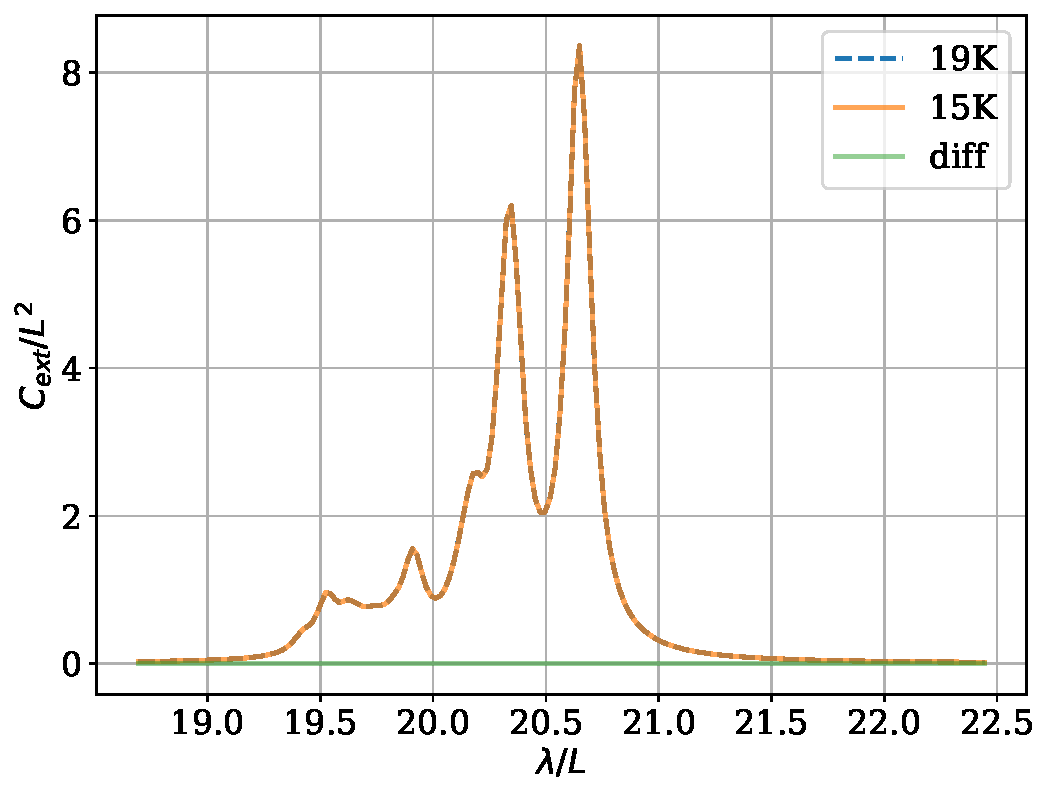
\includegraphics[width=0.85\textwidth]{cubeL535nm_15Kvs19K.pdf} 
    \caption{Extinction cross section divided by $L^2$ as a function fo wavelength divided by $L$ of
    a cube of size L=535 nm}
    \label{fig:cube535}
 \end{figure}
